\documentclass[final,t]{beamer}
\mode<presentation>{ \usetheme{Major} }
\usepackage{times}
\usepackage{amsmath,amsthm, amssymb, latexsym}
\boldmath
\usepackage[english]{babel}

\usepackage{relsize}
\usepackage{multirow}
\usepackage{qtree}
\usepackage{stmaryrd}
\usepackage{booktabs}

%  \usepackage[font=small,format=plain,labelfont=bf,up,textfont=it,up]{caption}
\usepackage[font=small,labelfont=small,bf,margin=2cm]{caption}
\usepackage[latin1]{inputenc}
\usepackage[orientation=landscape,size=a0,scale=1.4,debug]{beamerposter}
\usepackage{color,listings}
\usepackage{calc,xcolor}

\definecolor{lightblue}{rgb}{.85,.85,1} % 217 217 255
\definecolor{lightorange}{rgb}{1,.8,.6} % 255 204 153
\definecolor{lightgreen}{rgb}{.77,.91,.5} % 196 232 128
\definecolor{lightyellow}{rgb}{1,.98,.6} % 255 250 153


\newsavebox\CBox
\newenvironment{ColorBox}[3][black]{
    \par\noindent
    \def\borderColor{#1}\def\bgColor{#2}
    \begin{lrbox}{\CBox}
    \minipage{#3-2\fboxsep-2\fboxrule}
}{
    \endminipage\end{lrbox}%
    \fcolorbox{\borderColor}{\bgColor}{\usebox\CBox}\par
}

\lstset{language=java}
\lstset{breaklines=true}
\lstset{showstringspaces=false}
\lstset{tabsize=3}
\lstset{basicstyle=\ttfamily\scriptsize}
\lstset{breakautoindent=true}
\lstset{postbreak=\space}
%\lstset{commentstyle=\color{XcodeComments}}
%\lstset{keywordstyle=\color{XcodeKeywords}}
%\lstset{stringstyle=\color{XcodeStringstyle}}

%%%%%%%%%%%%%%%%%%%%%%%%%%%%%%%%%%%%%%%%%%%%%%%%%%%%%%%%%%%%%%%%%%%%%%%%%%%%%%%%%5
\title[]{An Underwater Robotic Smart-Sensing System for Water Quality Testing}
\author[Wright]{Elisia Wright and Dr. Janyl Jumadinova}
\institute{Department of Computer Science, Allegheny College}
\webpage{cs.allegheny.edu}
\mail{wrighte@allegheny.edu}

%%%%%%%%%%%%%%%%%%%%%%%%%%%%%%%%%%%%%%%%%%%%%%%%%%%%%%%%%%%%%%%%%%%%%%%%%%%%%%%%%5
\begin{document}
    \begin{frame}{}
        \vspace*{-6mm}
        \begin{columns}[t]

            %%%%%%%%%%%%%%%%%%%%%%%%%%%%%%%%%%%%%%%%%%%%%%%%%%%%%%%%%%%%%%%%%%%%%
            %
            % Left column - Context
            %
            %%%%%%%%%%%%%%%%%%%%%%%%%%%%%%%%%%%%%%%%%%%%%%%%%%%%%%%%%%%%%%%%%%%%%
            \begin{column}{.5\linewidth}

                %%%%%%%%%%%%%%%%%%%%%%%%%%%%%%%%%%%
                %
                % Project Objectives
                %
                %%%%%%%%%%%%%%%%%%%%%%%%%%%%%%%%%%%
                \begin{alertblock}{\textsc{Project Objectives}}
                    \vspace*{6mm}
                    Design, implement and test ... :
                    \begin{itemize}
                        \item
                        \item
                        \item
                    \end{itemize}
                    \vspace*{6mm}
                \end{alertblock}

                %%%%%%%%%%%%%%%%%%%%%%%%%%%%%%%%%%%
                %
                % Method
                %
                %%%%%%%%%%%%%%%%%%%%%%%%%%%%%%%%%%%
                \begin{block}{\textsc{Algal Blooms}}
                    \vspace*{6mm}
                    \begin{figure}
                        \includegraphics[scale = 0.18]{assets/algalbloom.jpg}
                        \caption{Great Lakes: October 9, 2011}
                    \end{figure}
                    \vspace*{6mm}
                \end{block}

                \begin{block}{\textsc{Design}}
                    \vspace*{6mm}
                    % \begin{figure}
                    %     \includegraphics[scale = 0.15]{assets/IMG_9097.JPG}
                    %     \caption{Soldering wires}
                    % \end{figure}

                    \begin{center}
                    \begin{figure}
                    \begin{tabular}{cc}
                    \includegraphics[scale = 0.15]{assets/IMG_9097.JPG}
                    \hspace*{5mm}
                    &
                    \includegraphics[scale = 0.47]{assets/IMG_2627.jpg}
                    \end{tabular}
                    \caption{Soldering wires \hspace{24mm} Drilling holes for sensors}
                    \end{figure}
                    \end{center}

                    \vspace*{6mm}
                \end{block}
            \end{column}

            %%%%%%%%%%%%%%%%%%%%%%%%%%%%%%%%%%%%%%%%%%%%%%%%%%%%%%%%%%%%%%%%%%%%%
            %
            % Right column - Outcomes
            %
            %%%%%%%%%%%%%%%%%%%%%%%%%%%%%%%%%%%%%%%%%%%%%%%%%%%%%%%%%%%%%%%%%%%%%
            \begin{column}{.5\linewidth}

                %%%%%%%%%%%%%%%%%%%%%%%%%%%%%%%%%%%
                %
                % System
                %
                %%%%%%%%%%%%%%%%%%%%%%%%%%%%%%%%%%%
                \begin{block}{\textsc{Robot}}
                    \vspace*{6mm}
                    \begin{figure}
                        \includegraphics[scale = 0.5]{assets/group_pic.jpg}
                        \caption{Different robot models}
                    \end{figure}
                \end{block}

                \begin{block}{\textsc{Sensors}}
                    \vspace*{6mm}
                    \begin{itemize}
                        \item pH, Conductivity, Dissolved Oxygen, Temperature
                    \end{itemize}
                    \begin{figure}
                        \centering
                        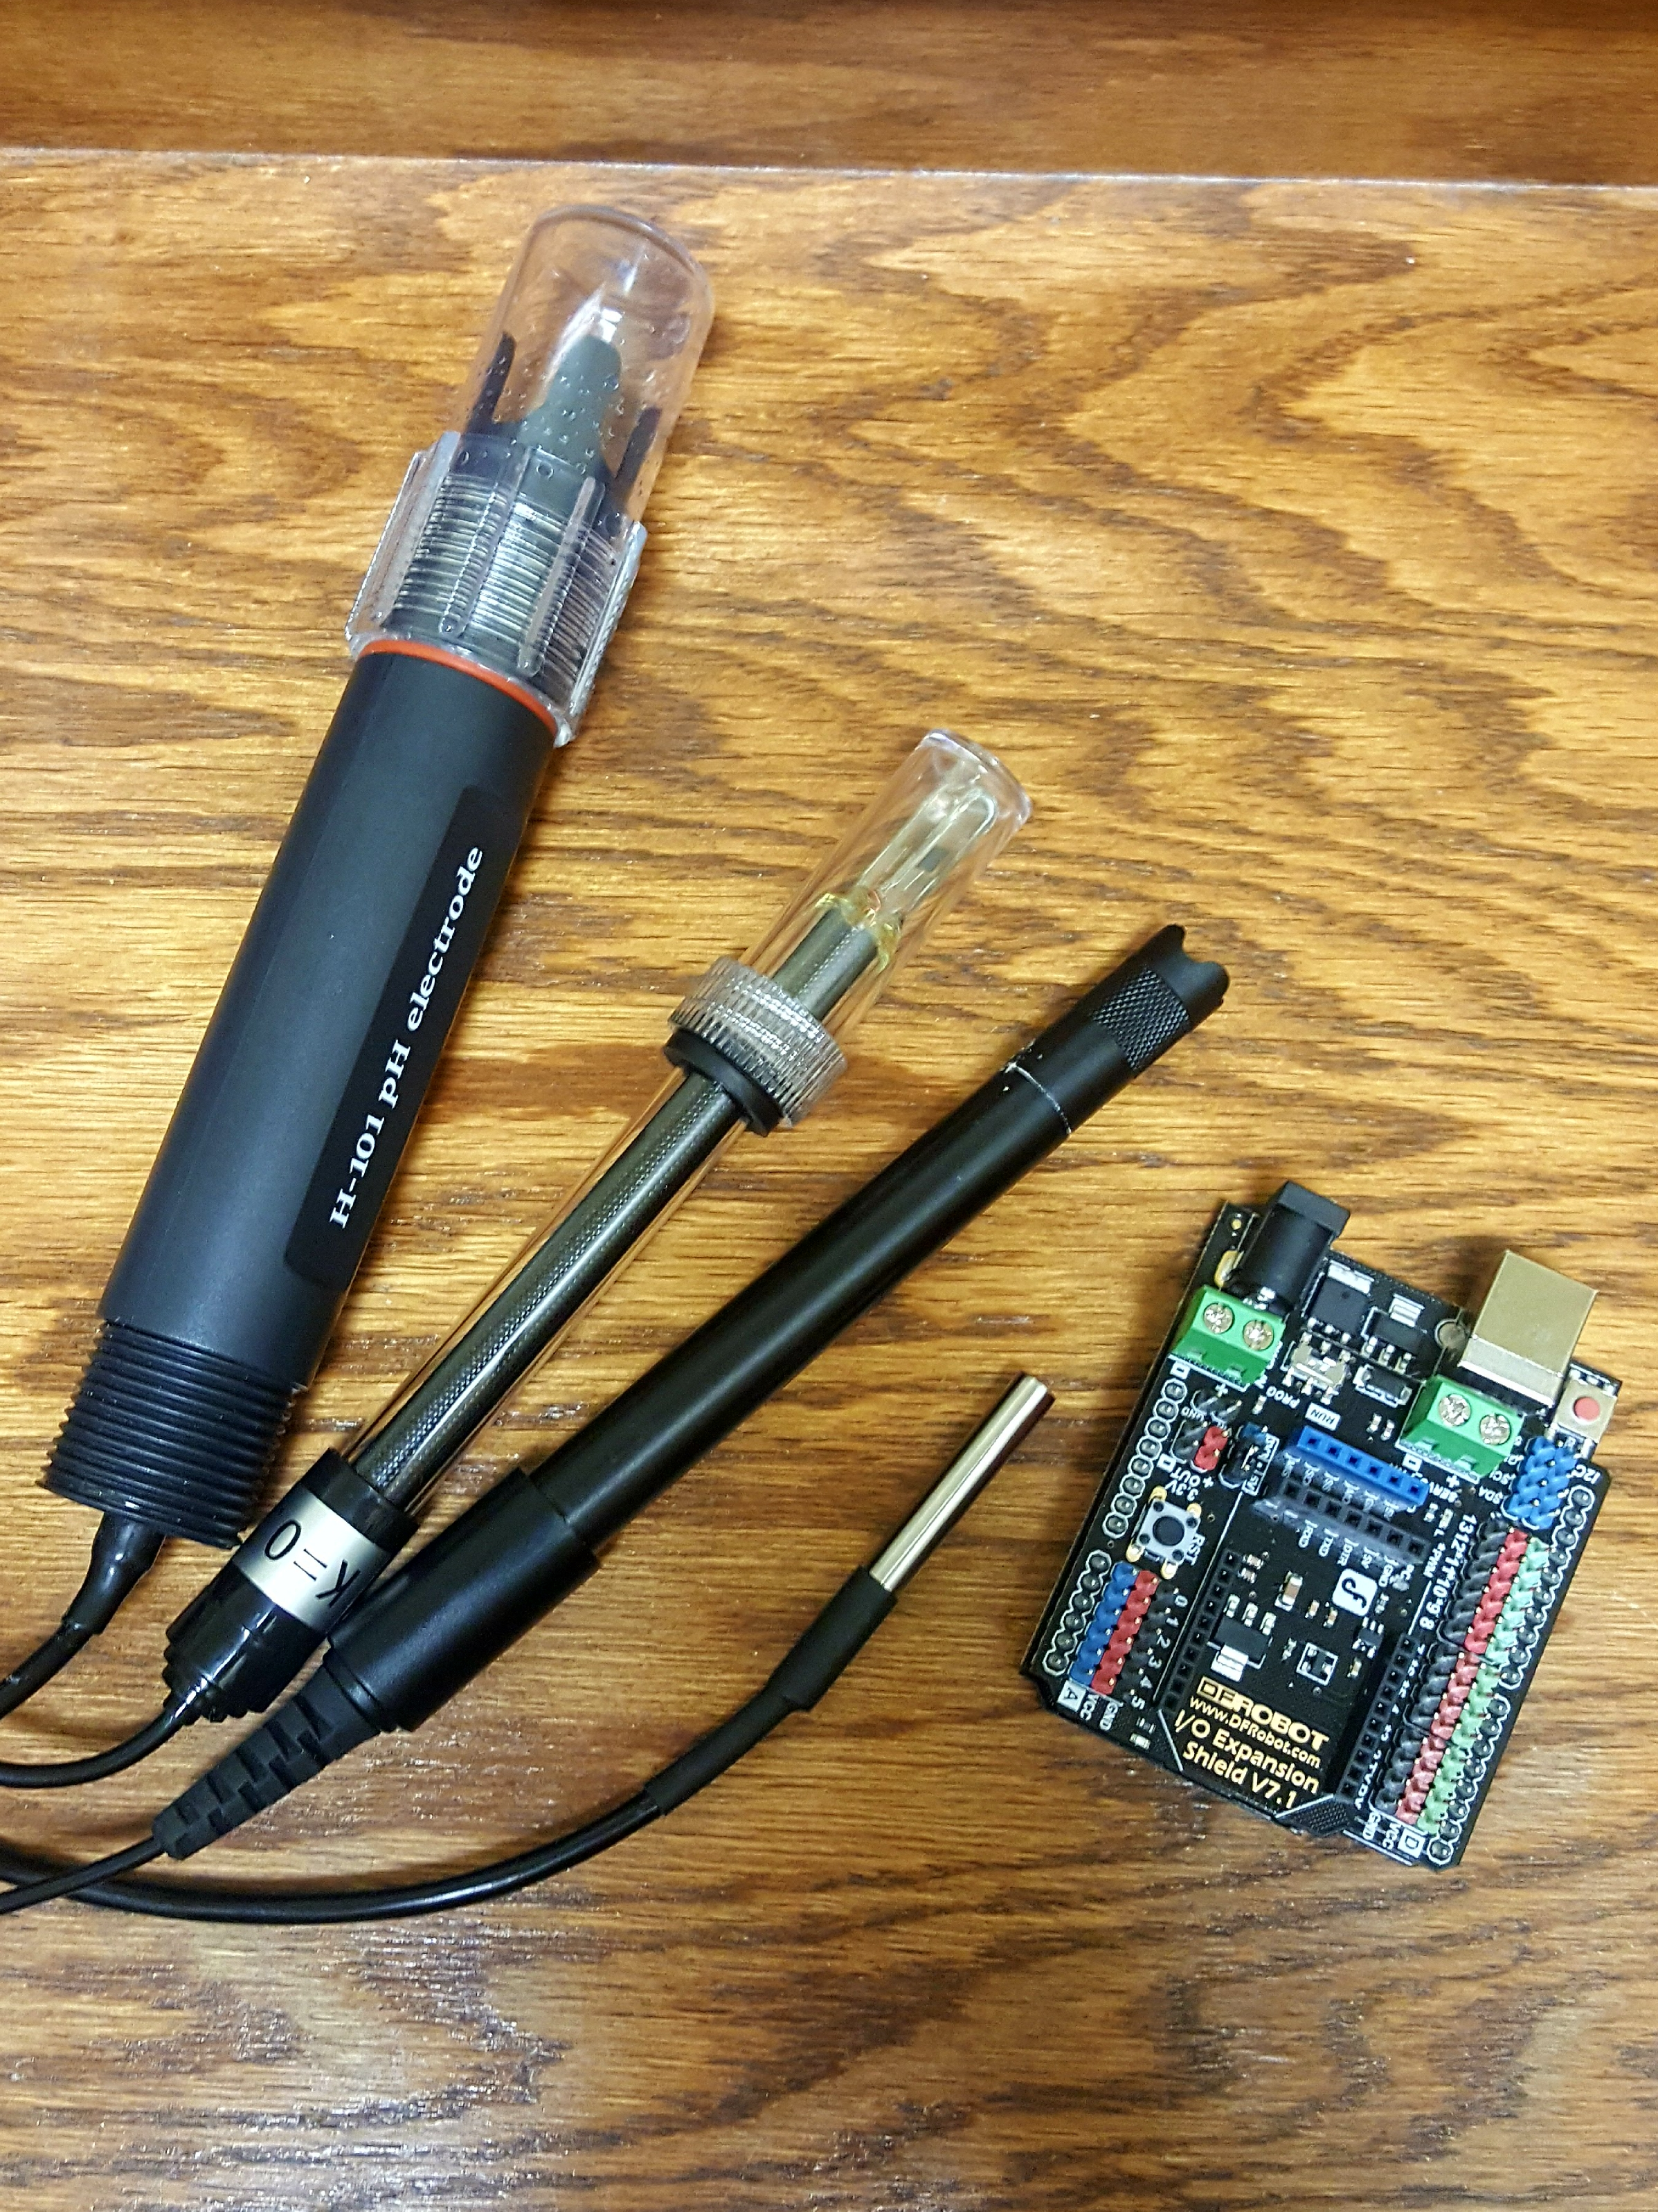
\includegraphics[scale = 0.2]{assets/sensors.jpg}
                        \caption{Arduino board and sensors}
                    \end{figure}
                \end{block}

                %%%%%%%%%%%%%%%%%%%%%%%%%%%%%%%%%%%
                %
                % Results
                %
                %%%%%%%%%%%%%%%%%%%%%%%%%%%%%%%%%%%
                \begin{block}{\textsc{Data}}
                    \vspace*{6mm}
                    % \begin{figure}
                    %     \includegraphics[scale = 2.5]{}
                    %     \caption{}
                    % \end{figure}
                \end{block}
            \end{column}


        \end{columns}
    \end{frame}
\end{document}
